%!TEX program = xelatex
\documentclass[12pt, a4paper]{report}
\usepackage[legalpaper, a4paper, margin=2cm]{geometry}
\usepackage[french]{babel}
\usepackage{hyperref}
\usepackage{libs/utbmcovers}
\usepackage{lipsum}
\usepackage{sectsty}
\usepackage{csquotes}
\usepackage[style=ieee]{biblatex}
\usepackage{fancyhdr}
\usepackage{tikz}
\usepackage{pdflscape}

%----------------------------------------
% Use Tahoma as base font
%----------------------------------------

\setmainfont{Tahoma.ttf}[
	Path=./assets/fonts/, 
	Extension=.ttf, 
	BoldFont = *Bold, 
	ItalicFont = *Italic, 
	BoldItalicFont = *BoldItalic,
	BoldSlantedFont = *BoldSlanted,
	SlantedFont = *Slanted,
	SmallCapsFont = *BoldSmallCaps,
]

\chapterfont{\tahomafont\fontseries{b}\fontsize{28pt}{36pt}}
\sectionfont{\tahomafont\fontseries{b}\fontsize{24pt}{28pt}}
\subsectionfont{\tahomafont\fontseries{b}\fontsize{20pt}{22pt}}
\subsubsectionfont{\tahomafont\fontseries{b}\fontsize{20pt}{22pt}}

%----------------------------------------
% UTBM covers configuration
%----------------------------------------

\setutbmfrontillustration{assets/images/utbm_default_illustration}
\setutbmtitle{REPORT TITLE 2}
\setutbmsubtitle{Internship Report ST40 - P2023}
\setutbmstudent{JACQUES Pierre-Paul}
\setutbmstudentdepartment{Computer Science Depertment}
\setutbmstudentpathway{IA - Artificial Intelligence}
\setutbmcompany{Company DEMO-Controlers}
\setutbmcompanyaddress{8 rue de la Fierté\\75 013 Paris}
\setutbmcompanywebsite{www.democontrollers.com}
\setutbmcompanylogo{assets/images/default_company}
\setutbmcompanytutor{COMPANY Tutor}
\setutbmschooltutor{SCHOOL Tutor}
\setutbmkeywords{
	[N°X – Y] Keyword 1,
	[N°X – Y] Keyword 2,
	[N°X – Y] Keyword 3,
	[N°X – Y] Keyword 4,
}
\setutbmabstract{ \lipsum[1-2] }

%----------------------------------------
% Document configuration
% Notes:
% - '\graphicspath' is used to add the path to the images.
% - '\addbibresource' is used to bibliographies files, use comma to add more than one.
%----------------------------------------

\graphicspath{{./assets/images/}}
\addbibresource{bibliography.bib}

%----------------------------------------
% Document
% Notes:
% - Usually, the abstract is not referenced in the table of contents
%	  nor the greetings section, so we use the '*' option to avoid it.
% - Non-cited references are not shown in the bibliography, so we use the
%	  '\nocite{*}' command to show them.
% - Everything below '\subsubsection' is not shown in the table of contents,
%----------------------------------------

\begin{document}
\tahomafont

% \makeutbmfrontcover{}

\topmargin -1.5cm
\pagestyle{fancy}
\fancyhf{}
\fancyhead[L]{
	\textbf{MR01: Méthodologie de recherche}
	\\ Présentation de votre programme de travail
}
% \fancyhead[R]{\thepage}
\fancyhead[R]{Julien Constant}
\renewcommand{\headrulewidth}{1pt}

% Présentation de votre programme de travail : identifiez les axes 
% de recherche, les grandes questions que vous vous posez sur votre 
% sujet et sur lesquelles vous allez rechercher de l’information 
% (vous pouvez utiliser mind view pour cela) ; carte en pdf à 
% déposer sur moodle, Avant le 08/10/2023

\begin{landscape}

\begin{figure}[h]
	\centering
	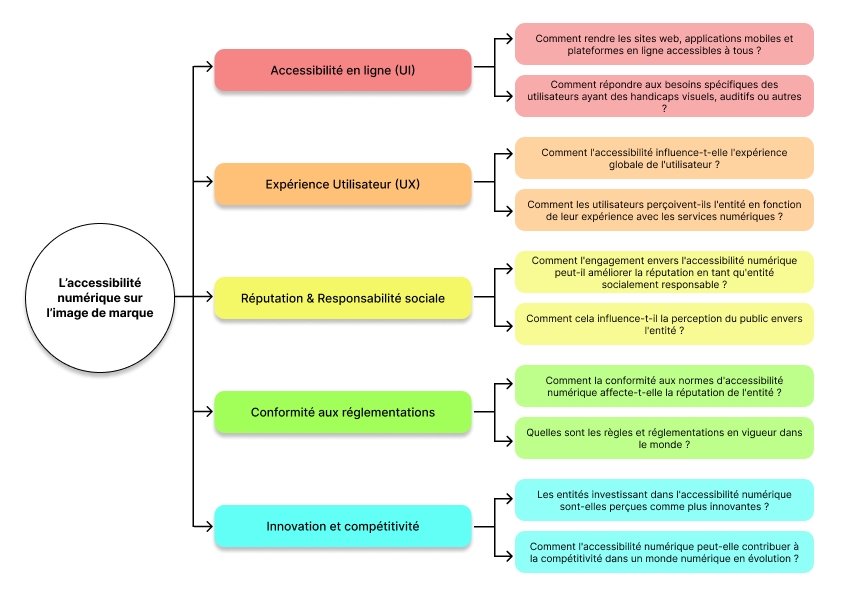
\includegraphics[width=1.4\textwidth]{assets/images/mindmap}
	\label{fig:mindmap}
\end{figure}

\end{landscape}

% \section*{Greetings}
% \lipsum[1-2] 

% \tableofcontents
% \newpage

% \chapter{Lorem Ipsum}
% \section{Section of Lorem Ipsum}
% \lipsum[1-1]\footnote{Footnote of Lorem Ipsum}

% \subsection{Sub Section of Lorem Ipsum}
% \lipsum[1-1]

% \subsubsection{Sub Sub Section of Lorem Ipsum}
% \paragraph{title of paragraph}
% \lipsum[1-1]

% \paragraph{}
% \lipsum[1-1]

% \newpage

% \nocite{*}
% \printbibliography{}

% \makeutbmbackcover{}
\end{document}